% !TeX root = resume.tex

\documentclass[10pt, a4paper]{article}

\usepackage{trimclip}
\usepackage{fontspec} % Для работы с системными шрифтами (нужен XeLaTeX или LuaLaTeX)
\usepackage{geometry} % Для настройки полей страницы
\usepackage{graphicx} % Для вставки изображений
\usepackage[svgnames]{xcolor} % Для работы с цветами
\usepackage{hyperref}   % для кликабельных ссылок
\usepackage{enumitem}   % для настройки списков
\usepackage{fontawesome5} % Для иконок (email, телефон и т.д.)
\usepackage{tikz}       % для рисования графических элементов (линия времени, кружки)
\usetikzlibrary{shapes.misc, positioning, arrows.meta}
\usepackage{changepage}

% --- НАСТРОЙКИ ШАБЛОНА ---

% 1. ГЕОМЕТРИЯ СТРАНИЦЫ
\geometry{
    a4paper,
    left=1.5cm,
    right=1.5cm,
    top=1.5cm,
    bottom=1.5cm,
    footskip=.5cm
}



% 2. ЦВЕТА
\definecolor{maintext}{HTML}{333333} % Основной цвет текста
\definecolor{graytext}{HTML}{666666} % Серый цвет для дат и подписей
\definecolor{boxgray}{HTML}{EBEBEB}  % Цвет для "таблеток" в интересах

% 3. ШРИФТЫ
\setmainfont{Lato} % Используем шрифт Lato. Убедитесь, что он установлен
\color{maintext}
\pagestyle{empty} % Убираем нумерацию страниц

% 4. НАСТРОЙКИ ССЫЛОК
\hypersetup{
    colorlinks=true,
    urlcolor=maintext,
    linkcolor=maintext,
    pdfborder={0 0 0}, % убираем рамку вокруг ссылок
}

\setlength{\parindent}{0pt}


\begin{document}
% !TeX root = ../resume.tex

% --- ВСПОМОГАТЕЛЬНЫЕ КОМАНДЫ ---

% Команда для заголовков секций (WORK EXPERIENCE, SKILLS и т.д.)
\newcommand{\sectiontitle}[1]{%
    \vspace{8pt}
    \par
    \noindent\MakeUppercase{#1}
    \hrule width 1\textwidth height 0.4pt
    \vspace{8pt}
}

% Команда для иконки внешней ссылки
\newcommand{\extlink}{\, \textcolor{graytext}{\faIcon{external-link-alt}}}

% Команда для пунктов в списке достижений
\setlist[itemize,1]{label=\,--, leftmargin=*, topsep=0pt, itemsep=4pt}

% Команда для описания языков
\newcommand{\languageskill}[2]{%
    \par\noindent\hangindent=1em\hangafter=0
    \makebox[8em][l]{#1} % Название языка
    \foreach \i in {1,...,5}{
        \ifnum\i > #2
            \tikz\draw[graytext, fill=white] (0,0) circle (2.5pt);
        \else
            \tikz\fill[maintext] (0,0) circle (2.5pt);
        \fi
        \hspace{2pt}
    }
    \vspace{4pt}
}

% Команда для "таблеток" с интересами
\newcommand{\interesttag}[1]{%
    \tikz[baseline=(X.base)] \node[draw=graytext, rounded corners=3pt, inner sep=4pt, text=graytext] (X) {#1};
}

% ===============================================================
% ШАПКА (ИМЯ, ФОТО, КОНТАКТЫ)
% ===============================================================

\begin{minipage}[t]{0.6\textwidth} % Левая часть шапки
    \begin{minipage}[c]{0.25\textwidth}
        \begin{tikzpicture}
            \clip (0,0) rectangle (\linewidth, \linewidth); % Определяем область видимости (квадрат)
            \node[
                inner sep=0pt, % убираем внутренние отступы
                path picture={
                    \node[
                        xshift=0, % сдвигаем фото влево
                        yshift=-30pt, % сдвигаем фото вверх
                    ] at (path picture bounding box.center) {
                        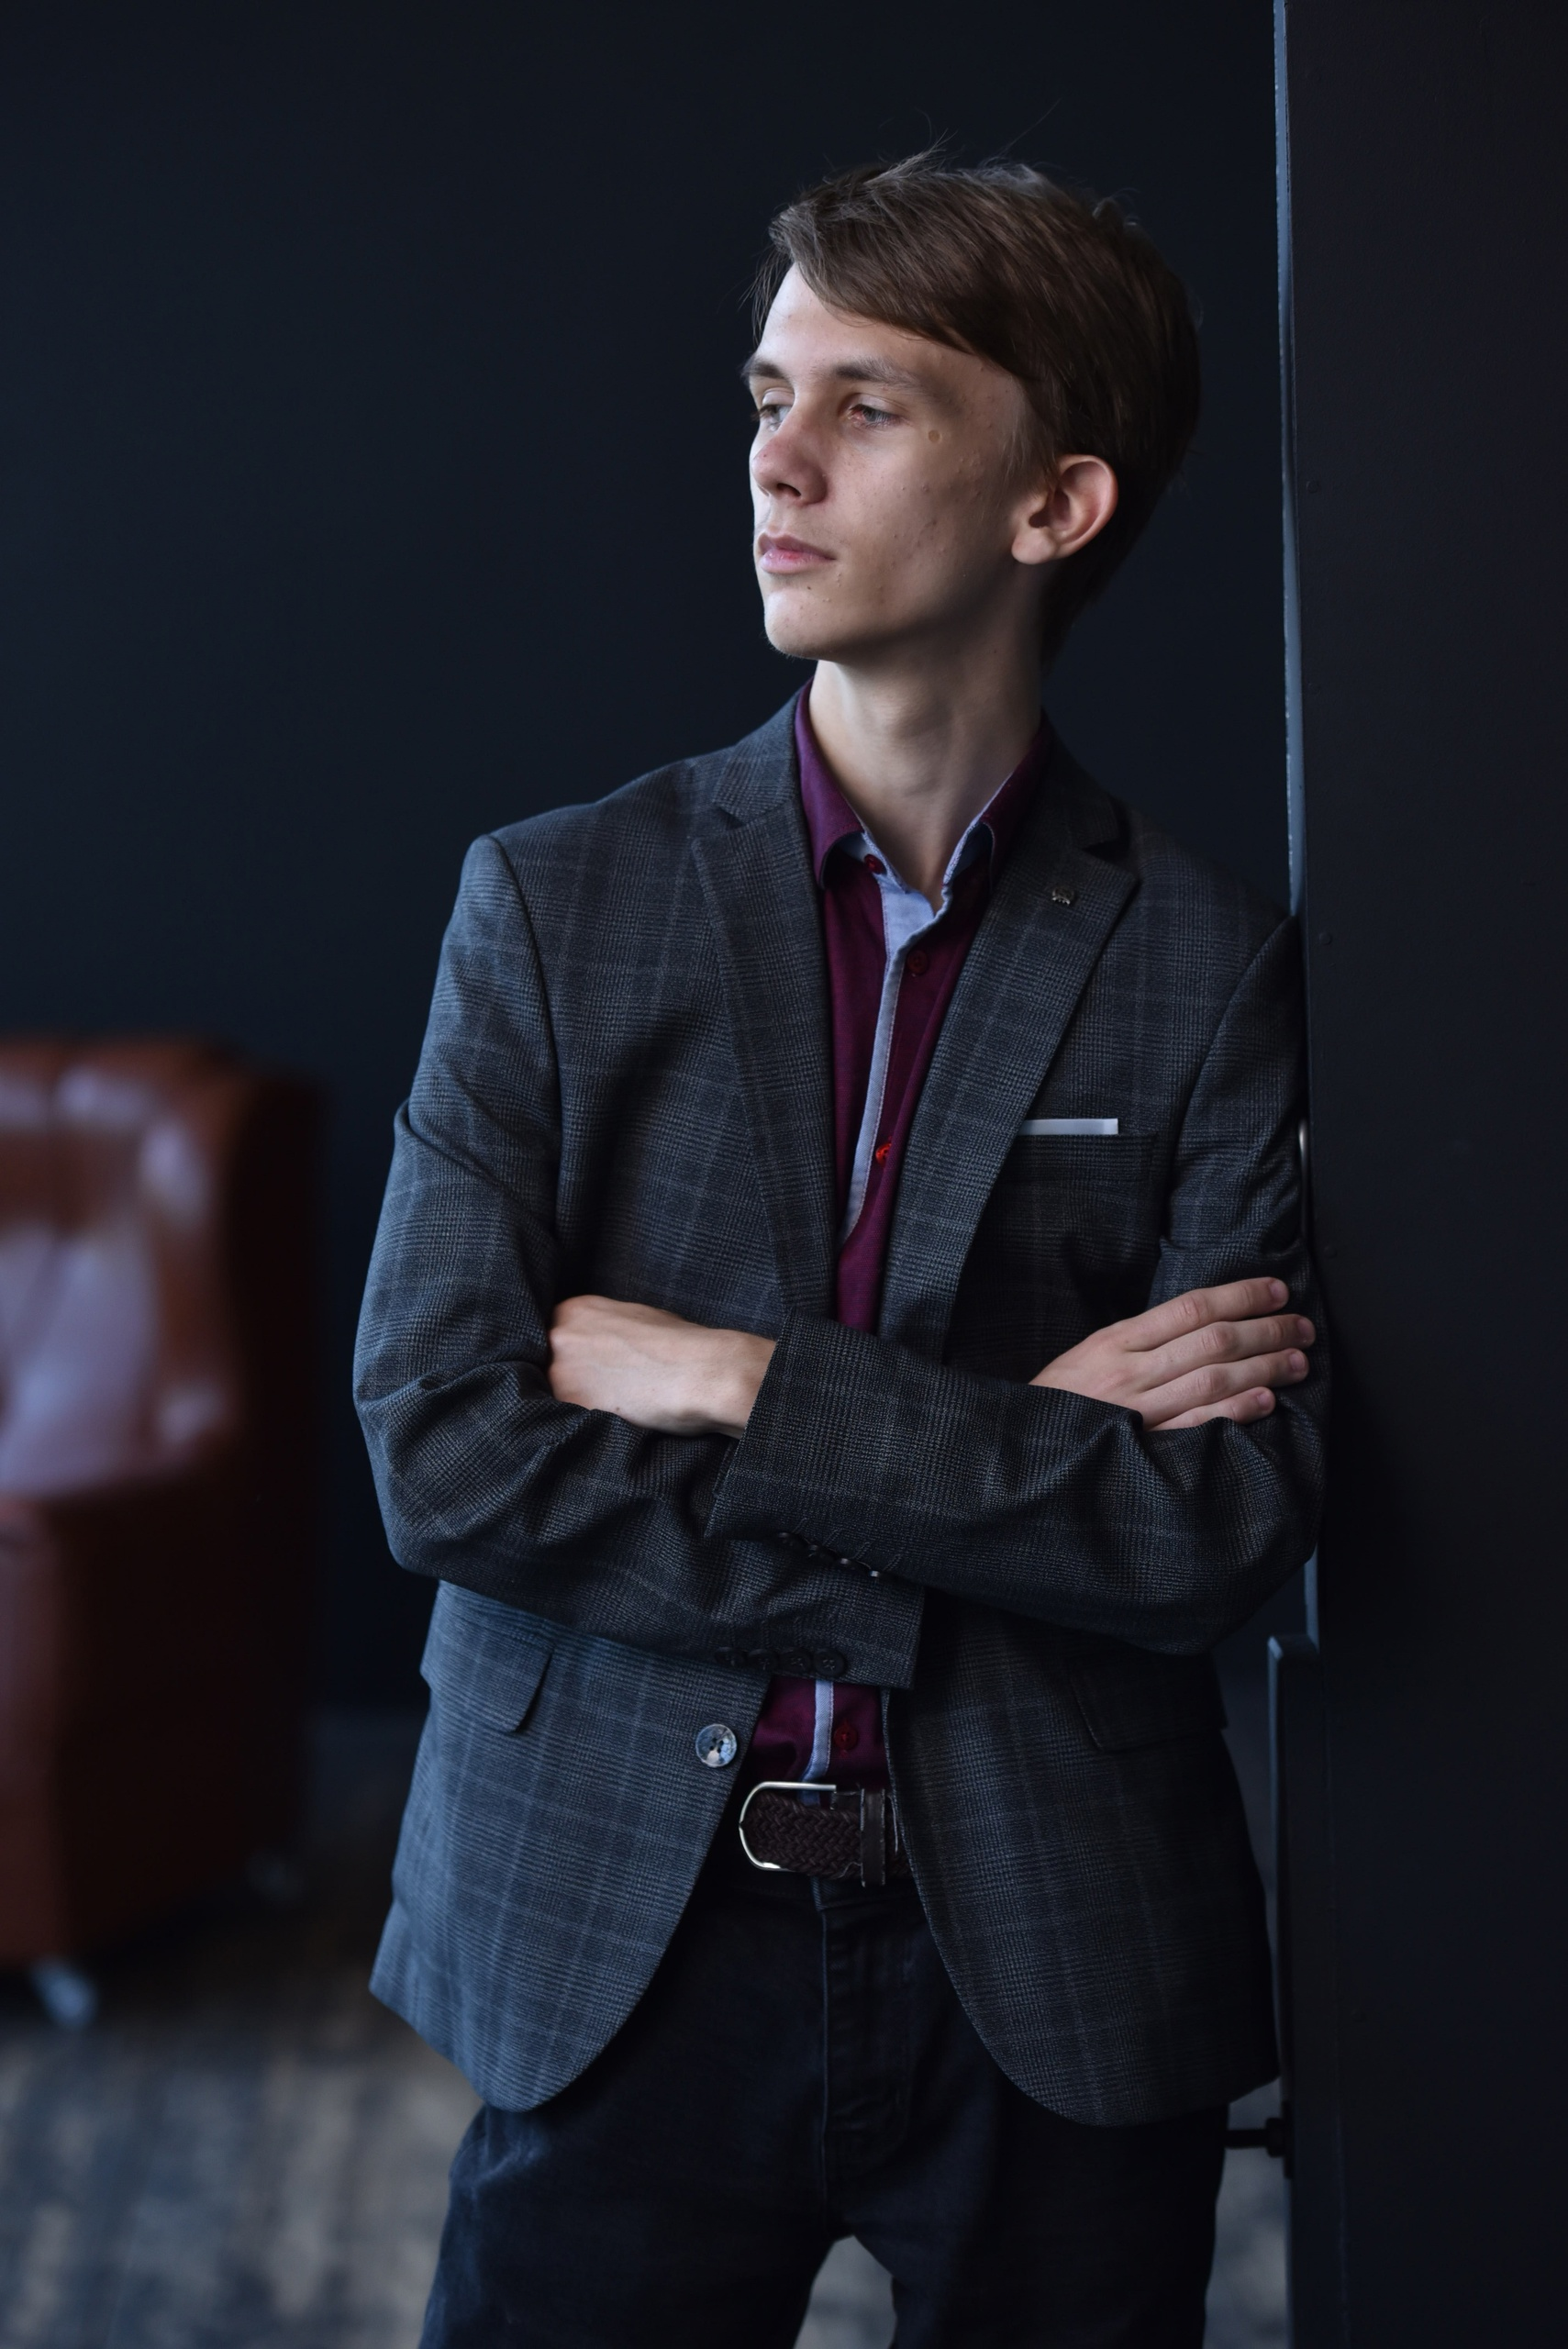
\includegraphics[width=1.2\linewidth]{self-photo.jpg}; % вставляем фото
                    };
                }
            ] at (0.5\linewidth, 0.5\linewidth) [draw=none, fill=none, minimum width=\linewidth, minimum height=\linewidth, rounded corners=15pt] {};
            % Рисуем рамку с закругленными углами, если нужно
            \draw[rounded corners=15pt] (0,0) rectangle (\linewidth, \linewidth);
        \end{tikzpicture}
    \end{minipage}%
    \hspace{0.02\textwidth} % Отступ между фото и текстом
    \begin{minipage}[c]{0.7\textwidth}
        \vspace{-1cm} % Подгонка по высоте
        \parbox{\linewidth}{
            \raggedright
            {\Huge \textbf{Sergey Novikov}}\\[5pt]
        }
    \end{minipage}
\end{minipage}%
\begin{minipage}{0.4\textwidth} % Правая часть шапки
    \raggedleft
    \small
    isnov.contact@gmail.com \faEnvelope \\[4pt]
    +7 (963) 571-66-95 \faIcon{mobile-alt} \\[4pt]
    Novosibirsk, RU \faIcon{map-marker-alt} \\[4pt]
    \href{https://github.com/Isn0v}{github.com/Isn0v} \faIcon{github} \\[4pt]
    \href{https://leetcode.com/u/Isn0v/}{LeetCode} \faIcon{code} \\[4pt]
\end{minipage}

\vspace{1.5cm}

% ===============================================================
% КРАТКАЯ СВОДКА (SUMMARY)
% ===============================================================
\noindent
A programmer with experience in teamwork. During my studies I developed some simple projects in cooperation with a team, sometimes taking the responsibility of organizing. Have a knowledge of C++, C, Go, Python and Java. I am learning system programming, actively studying DevOps tools and neural networks. I have practical experience with GitLab CI, as well as basic skills in Docker. I am highly adaptable, independent and sociable - I quickly master new technologies and effectively interact with the team without any problems or conflicts.

\vspace{1cm}

% ===============================================================
% ДВУХКОЛОНОЧНАЯ СТРУКТУРА
% ===============================================================

% Создаем две колонки: левая 70% ширины, правая 30%
\begin{minipage}[t]{0.6\textwidth}

\raggedright

% --- ОПЫТ РАБОТЫ ---
\sectiontitle{\faBriefcase \quad Work Experience}

\begin{tikzpicture}[remember picture]
    \node[circle, fill=maintext, inner sep=2.5pt] (c1) at (0,0) {};
\end{tikzpicture}
\hspace{0.5cm}
\begin{minipage}[t]{0.9\textwidth}
    \textbf{\Large Assistant Engineer} \\[2pt]
    \textcolor{graytext}{\href{https://rnew.tilda.ws/excelsiorathuawei}{Excelsior at Huawei}}\extlink \\
    \textcolor{graytext}{\textit{03/2025 - 07/2025}}
    \begin{itemize}
        \item \textbf{Developed} and implemented new features into existing GitLab CI/CD pipelines to automate build and deployment processes.
        \item \textbf{Optimized} the pipeline structure to reduce execution time and improve stability.
        \item \textbf{Improved} readability and maintainability of configurations, implemented best practices for describing jobs and stages.  
        \item \textbf{Documented} all changes and provided features.
    \end{itemize}
\end{minipage}

\vspace{1cm}

\sectiontitle{\faFolderOpen \quad Projects}

\begin{tikzpicture}[remember picture]
    \node[circle, fill=maintext, inner sep=2.5pt] (c1) at (0,0) {};
\end{tikzpicture}
\hspace{0.5cm}
\begin{minipage}[t]{0.9\textwidth}
    \textbf{\Large \href{https://github.com/B0GDANPN/BrickOS/tree/9-lab}{BrickOS}} \extlink \\[2pt]
    Simple implementation of an operating system core with interruption handling based on the Linux kernel and VGA text mode \\
\end{minipage}

\vspace{0.5cm}


\begin{tikzpicture}[remember picture]
    \node[circle, fill=maintext, inner sep=2.5pt] (c1) at (0,0) {};
\end{tikzpicture}
\hspace{0.5cm}
\begin{minipage}[t]{0.9\textwidth}
    \textbf{\Large \href{https://github.com/VolkovK04/NSTTF}{NSTTF (Not So Tiny Tensorflow)}} \extlink \\[2pt]
    Simple implementation of Tensorflow in C++ with support of GPU acceleration \\
\end{minipage}

\vspace{0.5cm}


\begin{tikzpicture}[remember picture]
    \node[circle, fill=maintext, inner sep=2.5pt] (c1) at (0,0) {};
\end{tikzpicture}
\hspace{0.5cm}
\begin{minipage}[t]{0.9\textwidth}
    \textbf{\Large \href{https://github.com/Isn0v/KeyLogger}{KeyLogger}} \extlink \\[2pt]
    Program in Windows with ability to log user's keystrokes, especially in Google Chrome Browser with further sending to mail server \\
\end{minipage}


\vspace{1cm}

% --- ОБРАЗОВАНИЕ ---
\sectiontitle{\faGraduationCap \quad Education}


\begin{tikzpicture}[remember picture]
    \node[circle, fill=maintext, inner sep=2.5pt] (c3) at (0,0) {};
\end{tikzpicture}
\hspace{0.5cm}
\begin{minipage}[t]{0.9\textwidth}
    \textbf{\Large Computer Science,} \\[2pt]
    \textit{\large System Programming} \\[4pt]
    \textcolor{graytext}{Novosibirsk State University} \\
    \textcolor{graytext}{Bachelor, \textit{2022 - 2026}}
\end{minipage}


\end{minipage}%
\hfill % Разделитель между колонками
\begin{minipage}[t]{0.35\textwidth}
\raggedright

% --- НАВЫКИ ---
\sectiontitle{\faCog \quad Skills}
\begin{minipage}[t]{0.45\textwidth}
    \small
    Linux \\[4pt]
    Algorithms and Data Structures \\[4pt]
    GitLab CI/CD \\[4pt]
    Git \& GitHub \\[4pt]
    C, C++, Go, Python, Java \\[4pt]
    CMake, Make \\[4pt]
    Parallel Programming \\[4pt]
    Network \\[4pt]
    Docker \\[4pt]
    SQL \\[4pt]
\end{minipage}%
\hfill
\begin{minipage}[t]{0.45\textwidth}
    \small
    Adaptability \\[4pt]
    Independence \\[4pt]
    Communication \\ [4pt]
    Teamwork \\[4pt]
    Collaboration \\[4pt]
    Organization \\[4pt]
\end{minipage}

% --- ЯЗЫКИ ---
\sectiontitle{\faGlobe \quad Languages}
\small
\languageskill{Russian}{5}
\languageskill{English}{3}


\end{minipage}

\end{document}